\documentclass[../main.tex]{subfiles}
\begin{document}

\chapter{Lecture 5 - 23-03-2020}

\section{Tree Classifier}

Supposed we groped a tree up to this point and we are wandering how to
grow it.
\\
$S$ Training set $(x_1,y_1)...(x_m,y_m)$, $x_1 \in X$
\\
\begin{figure}[h]
    \centering
    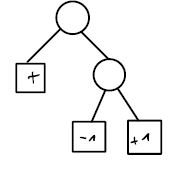
\includegraphics[width=0.4\linewidth]{../img/lez5-img1.JPG}
    \caption{Example of domain of $\knn$}
    %\label{fig:}
\end{figure}
\\
$$
\sll \equiv \{(x_1,y_1) \, x_t \quad \textit{is router to } \ell \}
$$
\\
$y_1 \in \{-1,1\}$
\\
$$
\sll ^+ \equiv \{(x_1,y_1) \in \sll : \quad y_t = +1 \} 
$$
$$
\sll^- \equiv \{(x_1,y_1) \in \sll : \quad  y_t = -1 \} 
\qquad
\sll^+ \cap \sll^- \equiv 0 \qquad \sll \equiv \sll^+ \cup \sll^-
$$

$$
\qquad \nl = | \sll| 
\qquad \nl^+ = |\sll^+| 
\qquad  \nl^- = |\sll^-| $$
$$
\nl = \nl^- + \nl^+
$$
leaf $\ell$ classifies all traning example ($\sll$)
\\
$$
Y_{\ell} = 
\begin{cases}
+1, & \mbox{If } \nl^+ \geq \nl^- 
\\
-1, & \mbox{If } otherwise
\end{cases}
$$
\\
$\ell$ makes a mistake on $min \{\nl^+, \nl^- \}$ example in $\sll$
$$
\hat{\ell}(h_T) = \frac{1}{m} 
\cdot \sum_{\ell}{} min \{ \frac{\nl^+}{\nl} , \frac{\nl^-}{\nl} \} \cdot \nl =
$$
$$
= \frac{1}{m} \cdot \sum_{\ell}{}\psi \cdot (\frac{\nl+}{\nl}) \cdot \nl \quad \longrightarrow  \qquad \frac{\nl^+}{\nl} = 1 - \frac{\nl}{\nl ??}
$$
where $\psi(a) = min \{a, 1-a \} \qquad a \in [0,1] $
\\
I want to replace inner node with other leaves.
\\
\begin{figure}[h]
    \centering
    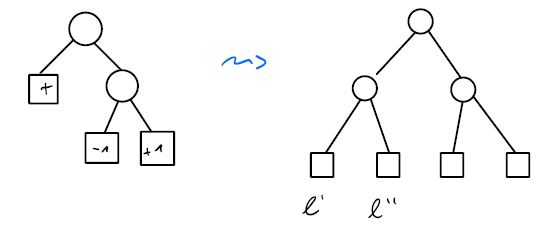
\includegraphics[width=0.8\linewidth]{../img/lez5-img2.JPG}
    \caption{Example of domain of $\knn$}
    %\label{fig:}
\end{figure}
\\
How is traning error going to change?
(when i replace inner nodes with other leaves)
\\
I’m hoping my algorithm is not going to overfit (if training error goes to 0 also
testing error goes to 0).
\newpage
\section{Jensen’s inequality}
If $\psi$ is a concave function $\longrightarrow $ (like $log$ or $\sqrt[2]{..}$ )
\\
\begin{figure}[h]
    \centering
    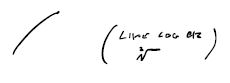
\includegraphics[width=0.4\linewidth]{../img/lez5-img3.JPG}
    \caption{Example of domain of $\knn$}
    %\label{fig:}
\end{figure}
\\
Also $\psi$ is a function that map $0$ to $1$, \quad $\longrightarrow$ \quad $\psi\:[0,1]\rightarrow \barra{R}$\\
$$
\psi(\alpha \cdot a + (1-\alpha) \cdot b ) \geq \alpha \cdot \psi(a) + (1-\alpha) \cdot \psi(b)
\qquad \textit{Also 2° derivative is negative}$$
\begin{figure}[h]
    \centering
    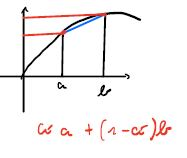
\includegraphics[width=0.5\linewidth]{../img/lez5-img4.JPG}
    \caption{Example of domain of $\knn$}
    %\label{fig:}
\end{figure}
\\
$$ \hat{\ell}(h_T) = \frac{1}{m} \cdot \sum_{\ell}{} \psi  (\frac{\nl^+}{\nl}) \cdot \nl
$$
\\
Look  a single contribution fo a leaf $\ell$ to training error
\\
$$
\psi(\frac{\nl^+}{\nl}) \cdot \nl = \psi(\frac{\nl'^+}{\nl'} \cdot \red{\frac{\nl'}{\nl}} + \frac{\nl"^+}{\nl"} \cdot \red{\frac{\nl"}{\nl}}) \cdot \nl
$$
where $\red{\frac{\nl'}{\nl}} = \alpha$ and $\red{\frac{\nl"}{\nl}} = 1-\alpha$ \qquad so \quad $\red{\frac{\nl'}{\nl}} + \red{\frac{\nl"}{\nl}} = 1$ \qquad $\longrightarrow$ $\alpha + 1 -\alpha = 1$
\\\\
$N_{\ell'}^+ + N_{\ell"}^+ = \nl
$ 
\\\\
I want to check function $min$ concave between 0 and 1.\\
$$min (0,1) = 0  \qquad \psi(a) = min(\alpha, 1- \alpha) $$
\begin{figure}[h]
    \centering
    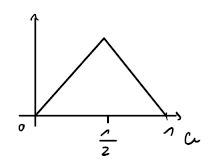
\includegraphics[width=0.4\linewidth]{../img/lez5-img5.JPG}
    \caption{Example of domain of $\knn$}
    %\label{fig:}
\end{figure}
\\
\red{This is a concave function and now I can apply Jensen's inquality}
\\\\
$$
\psi(\frac{\nl^+}{\nl}) \cdot \nl 
\geq 
(\frac{\nl'}{\nl} \cdot \psi (\frac{\nl'^+}{\nl'})
+ 
\frac{\nl"}{\nl}\cdot \psi(\frac{\nl"^+}{\nl"})) \cdot \nl =
$$

$\qquad \qquad\qquad \qquad \quad= $ 
\framebox[1.1\width]
{
$
\psi(\frac{\nl'^+}{\nl'})\cdot \nl'
+
\psi(\frac{\nl"^+}{\nl"})\cdot \nl"
$
}
\\\\
\red{This are the contribuion of $\ell'$ and $\ell"$ to the training error}
\\\\
Every time i split my tree my training error is never going to increase since we
have a concave function.\\
Whenever I’m growing my tree training error is going to be smaller.\\\\
\textbf{Every time a leaf is expanded the training error never goes up.
(Hopelly will go down)}
\\
I’ll should always grow the tree by expanding leave that decrease the training
error as much as possible.\\
If i take the effort of growing the tree i should get benefits. I can imaging that if
i grow the tree at random my training error is going to drop down error (but
maybe will derive overfitting).\\
For now is just an intuition since we will introduced statistical learning model.\\\\
Could be complicated and tree big may have 100 leave and there could be
many way of associating a test with that leaves.\\
I can spent a lot of time to select which leave is the best promising to split.\\
\begin{itemize}
\item Grow the tree by expanding leave that decrease the training error as much
as possible
\item In general we can assume:\\greedy algorithm at each step pick the pair leaf and test that cause
(approximative) the largest decrease in training error\\
\end{itemize}
In practise we want optimise this all the way since it’s time expensive. That’s
the approximately since we are not every time sure.
\\\\
--- MANCA PARTE ---
\\
\begin{figure}[h]
    \centering
    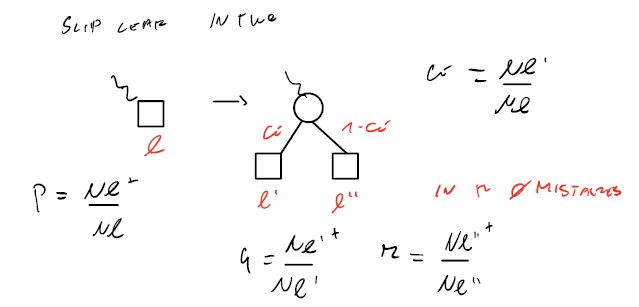
\includegraphics[width=0.8\linewidth]{../img/lez5-img6.JPG}
    \caption{Example of domain of $\knn$}
    %\label{fig:}
\end{figure}
\\
$ p = 0.8 \qquad q = 1 \qquad r = 1 \qquad \alpha = 60\%$
\\
Net Change in number of mistakes\\
$$
\psi(p) - (\alpha \cdot \psi(q) + (1- \alpha ) \cdot \psi (r) ) = 
$$
$$
\red{
\qquad \qquad  \ell \quad- \qquad \ell' \quad+ \qquad \ell" \qquad \qquad  \qquad \qquad 
}$$
Fraction of example miss classified $\ell -$ error $\ell' +$  error $\ell"$ \\
$$
= 0.2 - ( \frac{1}{2} \cdot 0.4 + \frac{1}{2} \cdot 0 ) = 0  
$$
\begin{figure}[h]
    \centering
    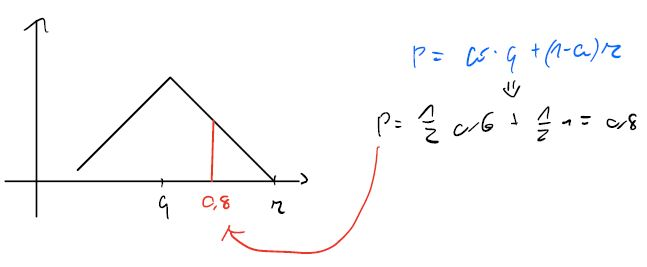
\includegraphics[width=0.6\linewidth]{../img/lez5-img7.JPG}
    \caption{Example of domain of $\knn$}
    %\label{fig:}
\end{figure}
\begin{figure}[h]
    \centering
    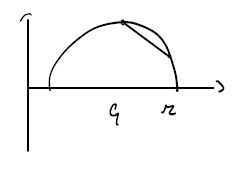
\includegraphics[width=0.4\linewidth]{../img/lez5-img8.JPG}
    \caption{Example of domain of $\knn$}
    %\label{fig:}
\end{figure}
\\
Idea is to replace minimum function with convex combination.
$$
\psi(\alpha) = min\ \{\alpha, 1-\alpha\} \qquad \psi(a) \geq \psi(\alpha)
$$
$$
\begin{cases}
\psi_1(\alpha) = 2\cdot\alpha \cdot (1-\alpha) \longrightarrow \red{GNI} \\
\psi_2(\alpha)= -\frac{\alpha}{2}\cdot \ln \alpha - \frac{1-\alpha}{2} \cdot \ln (1-\alpha)\longrightarrow \red{ENTROPY} \\
\psi_3(\alpha) = \sqrt[]{\alpha \cdot (1-\alpha
)}
\end{cases}
$$
All this functions has this shape (concave???)
\begin{figure}[h]
    \centering
    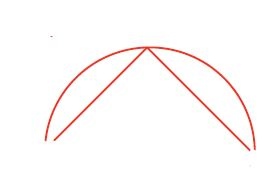
\includegraphics[width=0.4\linewidth]{../img/lez5-img9.JPG}
    \caption{Example of domain of $\knn$}
    %\label{fig:}
\end{figure}
\\
In practise Machine Learning algorithm use GNI or entropy to control the split
\section{Tree Predictor}
\begin{itemize}
\item Multi class classification $|Y| > 2$ $\longrightarrow$ \red{take majority}
\item Regression $Y = \barra{R} $ $\longrightarrow$ \red{take average of labels in $\sll$}
\end{itemize}
I still take majority among different classes.\\
Take average of labels in $\sll$
\\
Unless $\frac{\nl^+}{\nl} \in {0,1} $ \qquad $\forall$ leaves $\ell$, $\hat{\ell}(h_T) > 0$
\\
Unless leaves are \textit{"pured"}, the training error will be bigger than 0.
\\\\
In general, i can always write $\hat{\ell}(h_t)$ to 0 by growing enough the tree unless there are $x_1$ in the Time Series such that $(x_t, y_t)(x_t,y_t’)$ with $y_t \neq y_t’$ both occur.
\\
\begin{figure}[h]
    \centering
    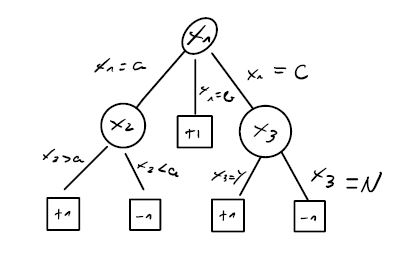
\includegraphics[width=0.7\linewidth]{../img/lez5-img10.JPG}
    \caption{Example of domain of $\knn$}
    %\label{fig:}
\end{figure}
\\
$$ if (x_1 = \alpha) \wedge (x_2 = \geq \alpha) \vee (x_1 = b) \vee (x_1 = c) \wedge (x_3= y) \qquad 
$$
$$
\textit{then predict 1} \qquad \qquad
$$
$
\qquad \quad \,\,else
$
$$
\textit{then predict -1} \qquad \qquad
$$
\\
--- Picture of tree classifier of iris dataset. ---\\
I’m using due attribute at the time.\\
Each data point is a flower and i can measure how petal and sepal are long.
I can use two attribute and i test this two. I can see the plot of the tree
classifier (second one) making test splitting data space into region that has
this sort of “blackish” shape ( like boxes: blue box, red box, yellow box)\\
A good exercise in which I want to reconstruct the tree given this picture.
\\\\
\section{Statistical model for Machine Learning}

To understand Tree classifier, nearest neighbour and other algorithm...\\
It’s important to understand that the only way to have a guideline in which
model to choose.\\\\
\textbf{This mathematical model are developed to learning and choose learning
algorithm.}\\\\
Now let start with theoretical model.
\begin{itemize}
\item How example $(x,y)$ are generated to create test set and training set?\\
We get the dataset but we need to have a mathematical model for this
process.
$(x,y)$ are drawn from a fixed but unknown probability distribution on the pairs $X$
and $Y$ ($X$ data space, $Y$ label set o label space)
\item Why $X$ should be random? \\
In general we assumed that not all the $x$ in $X$ are equally likely to be observed.
I have some distribution over my data point and this said that I’m most like to
get a datapoint to another.
\item How much label?\\
Often labels are not determined uniquely by their datapoints because labels
are given by human that have their subjective thoughts and also natural
phenomena. Labels are stochastic phenomena given a datapoint: i will have a
distribution.
\end{itemize}
We’re going to write (in capital) $(X, Y)$ since they are random variable drawn
from $D$ on $X \cdot Y$
A dataset $(X_1, Y_1) ... (X_m, Y_m)$ they are drawn independently from $D$
(distribution on examples)\\
When I get a training the abstraction of process collecting a training set\\
$D$ is a joint probability distribution over $X\cdot Y$\\
where $D_x$ is the marginal over $X \rightarrow D_y|x$ (conditional of $Y$ given $X$).\\
I can divided my draw in two part.
I draw sample and label from conditional.??\\
Any dataset ( training or test ) is a random sample (campione casuale) in the
statistical sense $\longrightarrow$ so we can use all stastical tools to make inference.
\end{document}